


{  \setbeamercolor{background canvas}{bg=sectioncolor}
\begin{frame}{Library: \code{xymbolyco}}{Deterministic Finite Automata}
  \centering
  %%By Photographer: Blake Griffin - Finite Automata and Dom Price, CC BY-SA 3.0, https://en.wikipedia.org/w/index.php?curid=47875021
  
\includegraphics[width=0.7\textwidth]{fa-band.jpg}
\end{frame}
}

\begin{frame}{DFA}{What are Finite Automata?}
  % https://medium.com/learning-data/understanding-algorithmic-time-efficiency-in-sql-queries-616176a85d02
  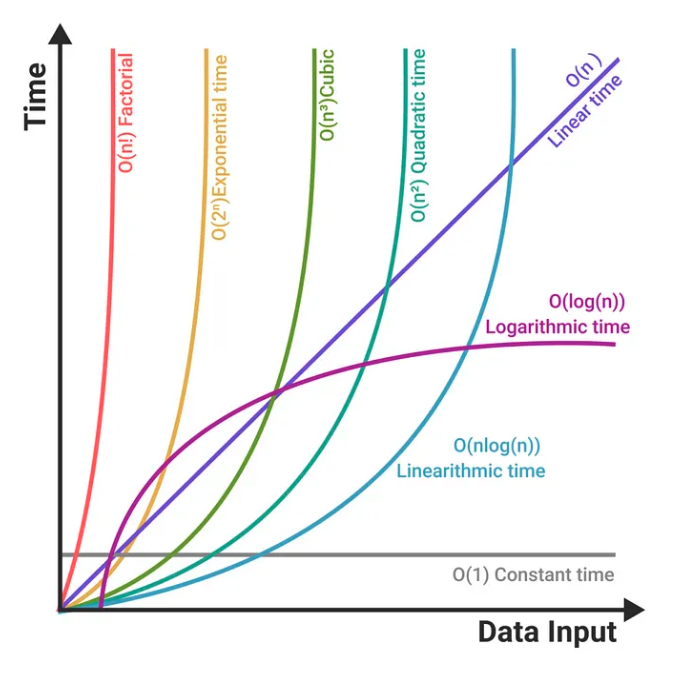
\includegraphics[width=0.4\textwidth]{complexity.png}

  \begin{itemize}
  \item   Every RTE corresponds to a Deterministic Finite Automata (DFA), \code{Rte.toDfa(rte)}, \Emph{$O(2^n)$}.

  \item   The DFA recognizes a sequence matching the RTE, \Emph{$O(n)$}.

  \end{itemize}
\end{frame}

\begin{frame}{\code{SimpleTypeD} Transitions}

  \scalebox{0.8}{\documentclass{standalone}
  \usepackage{tikz}
  \usetikzlibrary{arrows.meta, automata, bending, positioning, shapes.misc}
  \tikzstyle{automaton}=[shorten >=1pt, >={Stealth[bend,round]}, initial text=]
  \tikzstyle{accepting}=[double]

\begin{document}
\begin{tikzpicture}[automaton, auto]
  \node[state,initial,rounded rectangle] (0) {$0$};
  \node[state,rounded rectangle] (1) [right=20mm of 0] {$1$};
  \node[state,accepting,thick,rounded rectangle] (2) [above right=7mm and 30mm of 1] {$2$};
  \node[state,accepting,thick,rounded rectangle] (3) [below right=7mm and 30mm of 1] {$3$};
  \path[->] (0) edge node {$Int$} (1);
  \path[->] (1) edge[bend left=15]  node[pos=.8] {$Number \cap~!Int$} (2);
  \path[->] (1) edge[bend right=15] node[swap] {$String \cup Boolean$} (3);
  \path[->] (2) edge[bend left=15]  node {$Int$} (1);
  \path[->] (2) edge[loop above]    node {$Number \cap~!Int$} (2);
  \path[->] (3) edge[bend right=15] node[swap] {$Int$} (1);
  \path[->] (3) edge[loop below]    node {$String \cup Boolean$} (3);
\end{tikzpicture}
\end{document}
}

  A DFA transition is labeled by a \code{SimpleTypeD}.
\end{frame}



\begin{frame}{Uses of DFA}
  DFAs can be combined by an algebra.

  \begin{itemize}
  \item intersect RTE languages via intersecting the DFAs
  \item determine equivalence (or subset-ness) of two RTEs
  \item determine habitation and vacuity
  \item extract RTE from DFA
  \end{itemize}
\end{frame}


\begin{frame}{Demo}{Sample Flow}
  \centering
   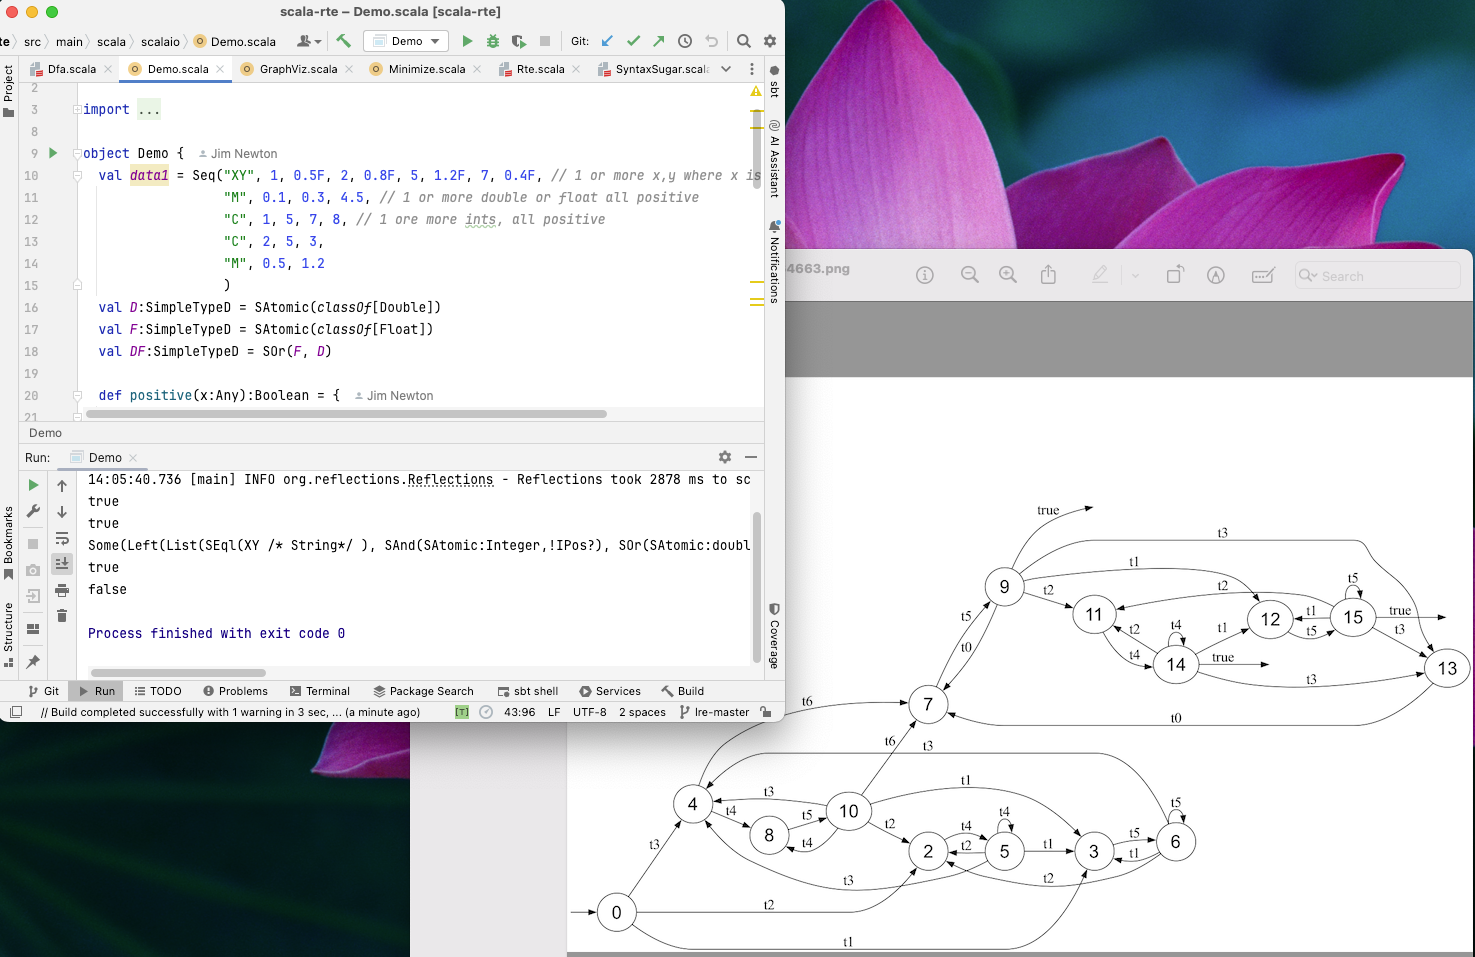
\includegraphics[height=0.8\textheight]{demo.png}
\end{frame}


\begin{frame}{Demo}{Sample Flow}
  Decide whether two RTEs are equivalent, and if not what is the difference.

  \code{ScalaIo2024.scala}

  \begin{itemize}
  \item define data
  \item define types and RTEs
  \item define two candidate patterns
  \item both match data
  \item show DFAs
  \item show xor DFA
  \item show spanning trace
  \end{itemize}

\end{frame}

